% IEEE standard conference template; to be used with:
%   spconf.sty  - LaTeX style file, and
%   IEEEbib.bst - IEEE bibliography style file.
% --------------------------------------------------------------------------
\documentclass[letterpaper]{article}
\usepackage{spconf,amsmath,amssymb,graphicx}
\usepackage[utf8]{inputenc}
\usepackage{listings}

% Example definitions.
% --------------------
% nice symbols for real and complex numbers
\newcommand{\R}[0]{\mathbb{R}}
\newcommand{\C}[0]{\mathbb{C}}

% bold paragraph titles
\newcommand{\mypar}[1]{{\bf #1.}}

\graphicspath{{figures/}}

% Title.
% ------
\title{Fast Implementation of Elliptic curve Diffie-Hellman}
%
% Single address.
% ---------------
\name{M.Gollub, C. Heiniger, T. Rubeli, H. Zhao}

\address{Department of Computer Science\\ ETH Z\"urich\\Z\"urich, Switzerland}

% For example:
% ------------
%\address{School\\
%		 Department\\
%		 Address}
%
% Two addresses (uncomment and modify for two-address case).
% ----------------------------------------------------------
%\twoauthors
%  {A. Author-one, B. Author-two\sthanks{Thanks to XYZ agency for funding.}}
%		 {School A-B\\
%		 Department A-B\\
%		 Address A-B}
%  {C. Author-three, D. Author-four\sthanks{The fourth author performed the work
%		 while at ...}}
%		 {School C-D\\
%		 Department C-D\\
%		 Address C-D}
%

\begin{document}
%\ninept
%
\maketitle
%

\begin{abstract}
Describe in concise words what you do, why you do it (not necessarily in this order), and the main result.  The abstract has to be self-contained and readable for a person in the general area. You should write the abstract last.
\end{abstract}

\section{Introduction}\label{sec:intro}
Cryptography is a complex and widespread computational problem in modern computer science research and applications. To ensure the confidentiality of the information exchange, encryption provides the core foundation of a secure information system. Among different cryptographic problems, key exchange is an essential topic for two distant users to be able to share a secret without meeting physically. Internet technology companies are interested in efficient yet high performance algorithms to fulfill the needs of exchanging keys in this age where network security has been concerned more than ever. Various key exchange protocols have been generated. Elliptic Curve Cryptography (ECC) has shown its advantages over traditional RSA (Rivest, Shamir and Adleman). By using less key sizes, ECC can apply a more efficient method without reducing the secure level of the encryption, whereas RSA requires the involvement of larger primer number to reach the same goal \cite{Malik:2010}.

As an important application domain of ECC, Elliptic Curve Diffie-Hellman (ECDH) key exchange has attracted researcher's attention due to its safety and efficiency. Diffie-Hellman scheme is a key agreement scheme that can provide implicit key authentication\cite{Brown:2009} and exchange shared secrecy. A fast implementation of ECDH is highly in demand, as the number of Internet users increases drastically with the growing needs for information security and the speed of computation. ECDH is widely used and there are some potential to be improved in its computational performance among the existed implementations. The challenge lies in the complex computational models and its natural requirements for large integers. In this paper, we propose a fast implementation of high performance ECDH key exchange.By comparing with popular cryptography library we proved the feasibility of our improvement of our optimization methods. 

Brown provides the backbone of this project by giving a general standard of Elliptic Curve Cryptography\cite{Brown:2009} and specifying a well-established deployment requirements\cite{Brown:2010}. Malik's work regarding a particular implementation in a FPGA card \cite{Malik:2010} shows the possibility of performance oriented optimization. The use of projective coordinates, as the most efficient optimization methods during our implementation, was proven by Blake et al.\cite{Blake:1999} as an effective method for expensive field inversions. OpenSSL is a world wide open source cryptography software which can fulfill the functionality for ECDH\cite{Emilia:2011}. In the end we can testify our optimization result by comparing our implementation with OpenSSL. In this paper we combine multiply approaches of optimizations and achieved satisfactory performance improvement and execution speedup.  

We give a thorough description of background in section 2, proposed optimization methods in section 3 and show our experimental results in section 4. In Section 5, we discuss and analyze our approach.

\section{Background: Elliptic curve Diffie-Hellman}\label{sec:background}
The purpose of this section is to familiarize the reader with the mathematical foundations of the Diffie-Hellman key exchange and which algorithms we used to achieve this task. This chapter follows a bottom-up approach.

\mypar{Finite Field arithmetic \cite[p. 3-4]{Brown:2009}} For elliptic curve cryptography one is mainly interested in the prime finite field $\mathbb{F}_p$ and the characteristic 2 finite field $\mathbb{F}_{2^m}$. In this paper only elliptic curves over $\mathbb{F}_p$ are discussed.

\mypar{Montgomery multiplication} 
\\The Montgomery modular multiplication algorithm allows to perform fast modular multiplication on large integers. In particular, the algorithm can be adapted for multi-precision arithmetic. Given two integers $x,y \in \mathbb{F}_p$, the algorithm computes $xy$ mod $p$. In order to perform the modular multiplication, $x$ and $y$ are converted to Montgomery form: $X = xR$ mod $p$ and $Y = yR$ mod $p$ where $R$ is larger than $p$ and co-prime with $p$. $R$ is usually chosen as $b^{t}$ where $b$ matches the size of a processor's word, $2^{64}$ in our case. The algorithm performs a chain of multiplication mod $b$ and division by $b$, which are simply mask and shift operations when $b$ is in the appropriate form. The algorithm for the multi-precision representation is given below \cite[p. 602]{Menezes:1996}


\begin{lstlisting}[frame=single, mathescape=true, captionpos=b, caption=Mulitprecision Montogmery Modular Multiplication ]
Input: 
p = ($p_{n-1}$ ... $p_{0}$)$_{b}$
X = ($x_{n-1}$ ... $x_{0}$)$_{b}$
Y = ($y_{n-1}$ ... $y_{0}$)$_{b}$

Output:
$XYR^{-1}$ mod $p$

1. A $\leftarrow$ 0 (A = ($a_n$ ... $a_{0}$)$_{b}$
2. for $i$ from $0$ to $(n-1)$ do:
	2.1 $u_{i} \leftarrow (a_{0}+x_{i}y_{0})p'$ mod $b$
	2.2 $A \leftarrow (A+ x_{i}y + u_{i}p) / b$
3. if $A \geq p$ then $A \leftarrow A-p$
4. return $A$
\end{lstlisting}

The challenging part of the reduction modulo $p$ resides in the high amount of division operations to be performed. The algorithm takes advantage of the underlying architecture by performing operations on machine words. The modulo operation in itself is only executed at the end, where $A$ is certain to be between $0$ and $2p-1$. (In the early phase of the project, we used a base $b=2$ for $R$). \emph{should be mentioned in section 3.}

\mypar{Shifting using vector instructions} 

The shift operation is used extensively in both our division and Montgomery multiplication algorithm. In the first implementation, we relied on multi-precision division which executes many shift-by-1-bit operations. Although the idea of using vector instruction can sound appealing, we did not see a major speed up when vectorizing the shift operation. The reason for this is that the shift needs to be performed across the vector and therefore also between two vector. This significantly slows the operation since the bits need to be moved between vectors but also across inner boundaries or vectors.

\mypar{Elliptic Curve over $\mathbb{F}_p$ \cite[p. 6-7]{Brown:2009}}
An elliptic curve is defined by the equation
\begin{equation}\label{eq:defining_eq_ec}
y^2 \equiv x^3 + ax + b \quad (\text{mod } p)
\end{equation}
where $p$ is an odd prime number and $a,b \in \mathbb{F}_p$ are the parameters of the curve. Furthermore $a, b$ need to satisfy $4a^3 + 27b^2 \not\equiv 0$. The elliptic curve $E\left(\mathbb{F}_p\right)$ consists of the Points $P=(x,y)$ $x,y \in \mathbb{F}_p$ satisfying (\ref{eq:defining_eq_ec}). Additionally we introduce $\mathcal{O}$ the so called point at infinity. The addition of points (affine coordinates) is defined as follows \cite{Brown:2009}
\begin{enumerate}
\item{$\mathcal{O} + \mathcal{O} = \mathcal{O}$}
\item{$(x,y) + \mathcal{O} = \mathcal{O} + (x,y) = (x,y) \quad \forall (x,y) \in E(\mathbb{F}_p)$}
\item{$(x,y) + (x,-y) = \mathcal{O} \quad \forall (x,y) \in E(\mathbb{F}_p)$}
\item{Assume  $x_1 \neq x_2$. $(x_1, y_1) + (x_2, y_2) = (x_3, y_3)$ is defined as $x_3 \equiv \lambda^2 - x_1 - x_2 \, (\text{mod } p),$ \\ $y_3 \equiv \lambda(x_1 - x_3) - y_1 \, (\text{mod } p)$ and $\lambda \equiv \frac{y_2 - y_1}{x_2 - x_1} \, (\text{mod } p)$}
\item{$(x_1, y_1) + (x_1, y_1) = (x_3, y_3)$ is defined as $x_3 \equiv \lambda^2 -2 x_1 \, (\text{mod } p)$, $\lambda (x_1 - x_3) - y_1  \, (\text{mod } p)$ and $\lambda \equiv \frac{3 x_1^2 + a}{2y_1} \, (\text{mod } p)$}
\end{enumerate}
Rule 4. describes how to add two different points whereas rule 5. explains how to double a point. The set of points satisfying (\ref{eq:defining_eq_ec}) and $\mathcal{O}$ together with this addition form a commutative group.

\mypar{Jacobian Coordinates  \cite[p. 59 - 60]{Blake:1999}}
"In cases where field inversions are significantly more expensive than multiplications, it is efficient to implement projective coordinates" \cite{Blake:1999} In Jacobian (also called projective) coordinates a point is represented as a triplet $(x,y,z)$ satisfying (\ref{eq:defining_eq_ec_jacobians}).
\begin{equation}\label{eq:defining_eq_ec_jacobians}
y^2 \equiv x^3 + axz^4 + bz^6 \quad (\text{mod } p)
\end{equation}
Point additions in jacobian coordinates do not need modular divisions in contrast to affine coordinates, as one can see in the rules 4 and 5. The formulas how to add points in jacobian coordinates can be found in \cite[p. 59-60]{Blake:1999}

\mypar{Double-and-add method}
In order to implement the Diffie-Hellman key exchange we need to calculate $dP$ fast.
\begin{lstlisting}[frame=single, mathescape=true, captionpos=b, caption=double-and-add method]
Input: $P \in E(\mathbb{F}_p)$, $d \in \mathbb{N}$
Output: $d\cdot P \in E(\mathbb{F}_p)$

$N$ $\leftarrow$ $P$
$Q$ $\leftarrow$ $\mathcal{O}$

for i from 0 to m do
  if $d_i$ = 1 then
    $Q$ $\leftarrow$ point_add($Q$, $N$)
  $N$ $\leftarrow$ point_double($N$)
return $Q$
\end{lstlisting}
where $d = d_0 + d_1 2 + ... + d_m 2^m \quad d_i \, \in \{0,1\}$

\mypar{Diffie Hellman key exchange \cite[p. 170-171]{Washington:2008}}
Alice and Bob want to establish a secret over a public channel. We assume that the elliptic curve parameter: a prime $p$, $a, b \in \mathbb{F}_p$ a point $G$ with high order are publicly known.
\begin{enumerate}
\item{Alice chooses a secret integer $u$, computes $G_u = uG$, and sends $G_u$ to Bob.}
\item{Bob chooses a secret integer $v$, computes $G_v = vG$, and sends $G_v$ to Alice.}
\item{Alice computes $uG_v = uvG$}
\item{Bob computes $vG_u = vuG$.}
\end{enumerate}
One can verify that $uG_v = uvG = vuG = v G_u$. An eavesdropper knows $G, G_u, G_v$ and his goal is to calculate $uvG$. This is known as the Diffie-Hellman Problem and is assumed to be a hard problem. 

\mypar{Complexity / Number of field operations}
Since in ECDH the essential operation is multiplying a Point with a scalar, we want to investigate the number of field operations when calculating $dP$. We assume the double-and-add method and Jacobian coordinates are used. This analysis is based on \cite[p. 63]{Blake:1999} As one can see in Listing \ref{lst:double_and_add} the number of point additions depends on the input $d$. Let $\ell$ be the number of bits of $d$. A reasonable assumption is to say, that $\ell / 2$ point additions and $\ell$ point doublings are necessary. Since arbitrary integer size multiplications are more expensive than additions we only count multiplications. According to \cite[p. 59, 60]{Brown:2009} a point addition costs 16 and a point doubling 10 multiplications. Hence we get an opcount of $\ell \cdot 10 + \ell / 2 \cdot 16$ multiplications.

\mypar{Cost measure}


\section{Implementation and optimizations}\label{sec:yourmethod}
The idea of this section is to give an overview about our implementation and the optimizations we did. We distinguish between four versions of our code. \textbf{Baseline}, which is the first naive implementation. \textbf{Memory optimization} uses the same algorithm as the baseline, but the memory handling is improved. The version \textbf{Jacobian coordinates} can be viewed as a second baseline, since a lot of algorithmic improvements were performed, which we figured out, when analyzing the OpenSSL implementation. \textbf{Final} marks our latest version.

\mypar{Baseline} 
Since we have to calculate with large numbers 64-bit integer operations are not sufficient. We therefore had to find a representation for arbitrary sized integers. We decided not to use a library, in order to have full flexibility in the optimizations. Our choice is shown in Listing \ref{lst:bigint}. As a next step we implemented the addition, shifting, modular multiplication and division. Furthermore we implemented Addition of points (affine coordinates) and multiplication of a Point with a scalar (double-and-add method). All of the functions were tested with unit tests.

\begin{lstlisting}[frame=single,  captionpos=b, caption=representation of the arbitrary size integers, label=lst:bigint]
typedef uint64_t block;

typedef struct 
{
    uint64_t significant_blocks;    
    block blocks[BIGINT_BLOCKS_COUNT]; 
} __BigInt;
\end{lstlisting}

\mypar{Memory optimization}

\mypar{First comparision with OpenSSL}
Realization that the chosen algorithm is not optimal.

\mypar{Jacobian coordinates}
Introduction of the Jacobian coordinates
Precomputation of the Points

\mypar{Final}
Final optimizations like function stitching and inline assembly 

Now comes the ``beef'' of the paper, where you explain what you
did. Again, organize it in paragraphs with titles. As in every section
you start with a very brief overview of the section.

For this class, explain all the optimizations you performed. This mean, you first very briefly
explain the baseline implementation, then go through locality and other optimizations, and finally SSE (every project will be slightly different of course). Show or mention relevant analysis or assumptions. A few examples: 1) Profiling may lead you to optimize one part first; 2) bandwidth plus data transfer analysis may show that it is memory bound; 3) it may be too hard to implement the algorithm in full generality: make assumptions and state them (e.g., we assume $n$ is divisible by 4; or, we consider only one type of input image); 4) explain how certain data accesses have poor locality. Generally, any type of analysis adds value to your work.

As important as the final results is to show that you took a structured, organized approach to the optimization and that you explain why you did what you did.

Mention and cite any external resources including library or other code.

Good visuals or even brief code snippets to illustrate what you did are good. Pasting large amounts of code to fill the space is not good.

\section{Experimental Results}\label{sec:exp}
To evaluate the optimization result, we benchmark the implementation on a 64 bit Arch Linux machine with a 3GHz Intel Skylake CPU i7-6600U. The throughput of 64 bit multiplication (mul, mulx) is 1 op/cycle, and throughput of 64 bit addition with carry (adc, adcx, adox) is 1 op/cycle. The peak performance is therefore 2 ops/cycle (6 Gops/s) on 1 core. GCC 6.1.1 is used with compile flags \texttt{-O3 -mavx2 -mbmi2 -madx}. 

Based on the recommended Elliptic curve parameters from the guidance standard \cite{Brown:2010}, we have chosen five predefined curves with various key sizes: 192, 224, 256, 384, 521 bits. All versions of the implementation have been validated by using Google Test and by checking the ECDH key exchange results. In the end we compare our implementation with OpenSSL \cite{openssl}, a well known open source library, to check our implementation effect. We linked our program to a locally compiled version of OpenSSL . 

\begin{figure}[h!]\centering
  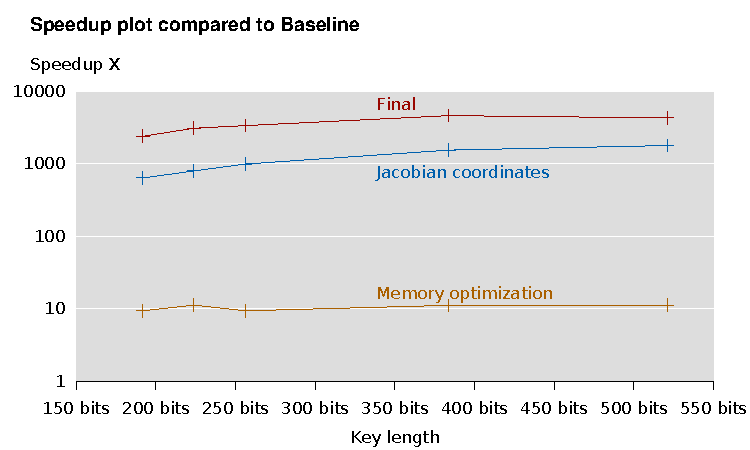
\includegraphics[scale=0.7]{speedup}
  \caption{Speedup plot compared to Baseline \label{speedup}}
\end{figure}
\begin{figure}[h!]\centering
  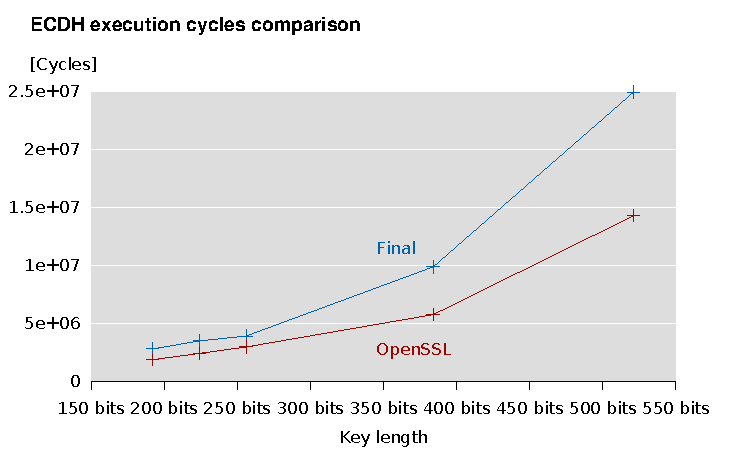
\includegraphics[scale=0.7]{ecdh}
  \caption{ECDH execution cycles comparison\label{ecdh}}
\end{figure}
\begin{figure}[h!]\centering
  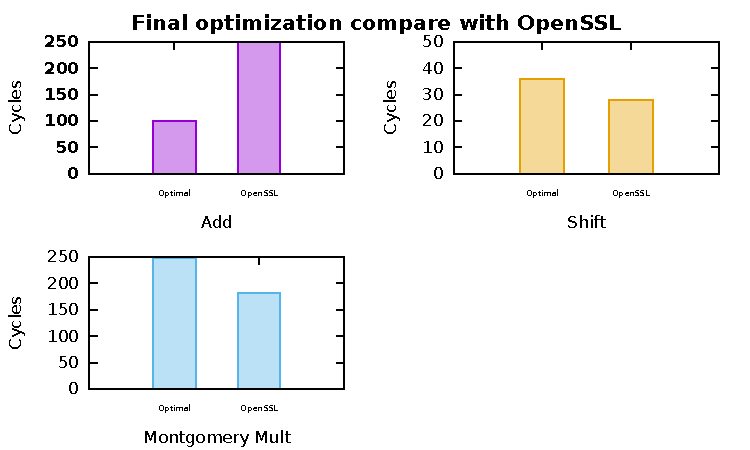
\includegraphics[scale=0.5]{openssl}
  \caption{Final optimization compared with OpenSSL\label{openssl}}
\end{figure}

In the speedup comparison (Fig.~\ref{speedup}) three crucial numbers are shown. It can be clearly seen that the Final implementation can execute the key exchange process 8900x faster than the baseline with the longest keys. The first milestone of memory optimization gives us about 10x speedup on average, whereas the Jacobian coordinates version of the code can run 1100x faster on average. This confirms the importance of the algorithmic changes explained in section \ref{sec:yourmethod}, including switching from projective to Jacobian coordinates. The resulting speedup is satisfactory and reasonable, as the first two versions of the implementation uses an inefficient memory management and a slower algorithm. The real performance boost is between the Jacobian coordinates and the Final version, after applying the architecture-specific optimizations mentioned in section 3. This gives us another 6x speedup on average, showing the efficiency of the final implementation.

Next we run the same operation using the OpenSSL library and compare the computation cycles (Fig.~\ref{ecdh}). Our number of required cycles remains the same level with OpenSSL, in key length range of less than 256 bits, yet falls behind OpenSSL with larger key length. Individual operations of integers are the main component of our algorithm. To see how good our implementation is we choose Montgomery multiplication to compare with OpenSSL (Fig.~\ref{openssl}). This comparison is done with the same input for both Final implementation and OpenSSL. Our implementation runs slightly behind OpenSSL. 

\begin{figure}[h!]\centering
  \includegraphics[scale=0.7]{perfplot1}
  \caption{Performance plot of baseline and memory optimization\label{perfplot1}}
\end{figure}
\begin{figure}[h!]\centering
  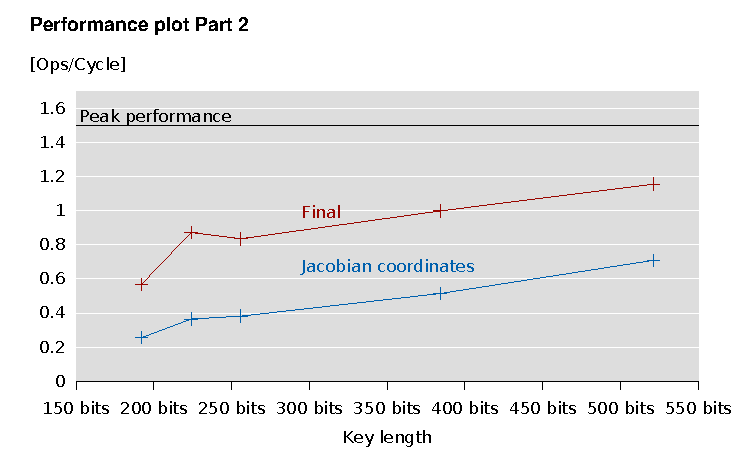
\includegraphics[scale=0.7]{perfplot2}
  \caption{Performance plot of Final optimization and Jacobian coordinates\label{perfplot2}}
\end{figure}

Performance plots (Fig.~\ref{perfplot1} and Fig.~\ref{perfplot2}) reflect if the implementation can make full use of the machines' computation ability. In Fig.~\ref{perfplot1} the first comparison is done by showing the effect of memory optimization. It is clear that with the bad memory management, the baseline performance is limited. The first approach of Memory optimization gives an increase of 4.17x in the largest key length and 4.1x in the smallest key length. In Fig.~\ref{perfplot2} we begin to see the real performance boost that comes from later optimization. Between these two figures the operation counts change drastically, thus we separate the performance plots. The peak performance here is calculated by considering the ratio of additions and multiplications. Considering the instruction balance in the main operation (Montgomery multiplication, 2 add : 1 mul), we can set the peak performance at 1.5 ops/cycle. As one can see, the final optimization are close to the peak performance with large key sizes. The highest performance of the final implementation is reached with $521$bit keys, with 1.41/1.5 = 94\% of the peak performance. From the Jacobian coordinates version to the Final we have a performance increase of 2.1x in the largest key length and 2.56x in the smallest key length. In all cases the performance increases as the key size grows. Relatively short key sizes, the setup time of the functions is relatively high compared to the time spent in the calculation loops. This prevents the program from reaching the peak performance. With longer keys the loops take most of the computation, bringing the program nearer to the peak performance.
\begin{figure}[h!]\centering
  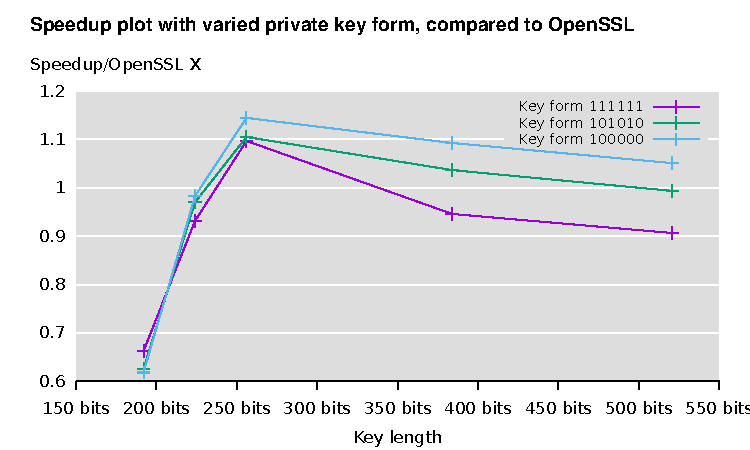
\includegraphics[scale=0.7]{keysize}
  \caption{Speedup plot with varied private key form, compared to OpenSSL\label{keysize}}
\end{figure}

Fig.~\ref{keysize} shows the our speedup compared with OpenSSL, depending on the form of the key. A key of the form 0b10..0 is optimal for the double-and-add method, since only one point addition has to be performed. Contrary to the form 0b11..1, which is the worst case scenario (see Listing \ref{lst:double_and_add}, lines 7,8). That can explain why in form 0b10..0 we are faster than OpenSSL and in form 0b11..1 we are slower. The runtime of OpenSSL seems to be independent of the key form. We assume this is a security measure for preventing side-channel attacks. So this has to be taken into consideration, when comparing the implementations.

\section{Conclusions}
In this project, we improved the performance of Elliptic Curve Diffie-Hellman key exchange with a C code implementation on an Intel CPU machine. It is proven by the experiments that the final optimization leads to better performance and faster execution time than the baseline. We also proposed a series of optimizing methods for large integer operations regarding Elliptic Curve Cryptography and combinations of testing approaches. It has also been shown that the final combined optimization achieves better result than the naive approach. Moreover, the final optimization does make the best use of Intel Intrinsics of the novel CPU model. 

Nevertheless, our approach is in general slightly behind the performance of OpenSSL and the form of private key will significantly influence the performance. Certainly there is still room to improve in this implementation. Execution time of larger key length set is one of the starting point. Since we use the base of 64 bits big integers, the total execution cycles are relatively high. Another significant limiting factor is the Montgomery multiplication, which is also the function that we are most behind compared with OpenSSL. Future work may include applying better shift algorithms and improving big integer structure.

% References should be produced using the bibtex program from suitable
% BiBTeX files (here: bibl_conf). The IEEEbib.bst bibliography
% style file from IEEE produces unsorted bibliography list.
% -------------------------------------------------------------------------
\bibliographystyle{IEEEbib}
\bibliography{bibl_conf}

\end{document}

